\chapter{Physical setup of the hydrodynamic computation}

In addition to the general setup given in the steering file, a number of
physical parameters may or should be specified upon a simulation.


\section{Hydrostatic pressure hypothesis}

Firstly, it should be specified whether one wants to use the hydrostatic
pressure hypothesis or not. That choice is made using the keyword
\telkey{NON-HYDROSTATIC VERSION} which, by default, is set to NO. As a
reminder, the hydrostatic pressure hypothesis consists in simplifying the
$W$ vertical velocity, ignoring the diffusion, advection and other
terms. Therefore, the pressure at a point is only related to the weight of the
overlying water column and to the atmospheric pressure at the surface. Without
the hydrostatic pressure hypothesis (\telkey{NON-HYDROSTATIC VERSION} = YES),
\telemac{3D} solves a $W$ vertical velocity equation which is similar to
the $U$ and $V$ equations, with the additional gravity term.


\section{Modelling turbulence}

The Reynolds numbers ($Re = U.L/\upsilon$) reached for tidal
flows or in an estuary are excessively high and illustrate basically turbulent
flows ($L$, the scale of eddies, for example, assumes the value of water
depth $h$ for a vertically homogeneous flow). For such a kind of flow,
the turbulence-induced momentum prevails (in relation to the molecular
diffusion). That diffusion is strictly defined by a tensor which could be
anisotropic.

The concept of eddy scale, however, is spatially constrained by the horizontal
and vertical scales of the modelled domain. At sea, for example, a one
kilometre long cape can generates eddies the dimensions of which are
horizontally related to that scale. Vertically, however, the eddy size is
constrained by the water depth or even more by possible effects of
stratifications. Synthetically, a common practice consists in separating the
vertical and horizontal turbulence scales which are not relevant to the same
dynamics for the standard applications of \telemac{3D}. That involves defining
horizontal as well as vertical viscosities rather than a single viscosity. On
the open sea, for instance, the horizontal and vertical viscosities differ by
several orders of magnitude.

Thus, the implementation of \telemac{3D} requires defining two models of
horizontal and vertical turbulence (\telkey{HORIZONTAL TURBULENCE MODEL},
\telkey{VERTICAL TURBULENCE MODEL}).

Turbulence modelling is an awkward task and \telemac{3D} offers the user several
approach options which are different, but also increasingly complex, and are
applicable to velocities as well as to active and passive tracers.

The Von Karman constant and Prandtl number (ratio between eddy viscosity and
eddy diffusivity) can be changed with the keywords \telkey{KARMAN CONSTANT}
(default value = 0.4) and \telkey{PRANDTL NUMBER} (default value = 1.).

\subsection{Constant viscosity}

The simplest turbulence model consists in using a constant viscosity
coefficient (option for parameters: 1="CONSTANT VISCOSITY", default value). In
that case, the latter includes the effects of molecular viscosity and
dispersion (refer to Theoretical note \cite{Hervouet2007}).
The horizontal and vertical
turbulent viscosities are then constant throughout the domain. The global
(molecular + turbulent) viscosity coefficients are provided by the user by
means of the keywords \telkey{COEFFICIENT FOR HORIZONTAL DIFFUSION OF
VELOCITIES} and \telkey{COEFFICIENT FOR VERTICAL DIFFUSION OF VELOCITIES}, set
by default to $10^{-6}$.

The value of that coefficient has a definite effect on both size and shape of
the recirculations and eddies. A low value will tend to only dissipate the
small-sized eddies, a high value will tend to dissipates large-sized
recirculations. The user shall then carefully select that value according to
the case studied. Usually, that value becomes a model calibration data by
comparison with measurements. Besides, it is worth mentioning that a value
bringing about the dissipation of recirculations of a smaller than two mesh
cell extent has nearly no influence on the computation (i.e. there is a
threshold beyond which the viscosity or turbulence value has substantially no
effect).

\telemac{3D} makes it possible to get a space- and time-variable coefficient.
The \telfile{VISCOS} subroutine will necessarily be programmed.
Within that subroutine, geometrical information, basic hydrodynamic
information (water depth, velocity components) and time are made available
to the user.

That option theoretically aims at enabling the user to define the turbulent
viscosity by programming the  \telfile{VISCOS} subroutine.

\subsection{Mixing length (vertical model)}

The user also has the opportunity to use a vertical mixing length model
(\telkey{VERTICAL TURBULENCE MODEL}: 2="MIXING LENGTH"). The vertical
diffusivity of velocities is then automatically computed by \telemac{3D} by means
of the selected mixing length model taking or not taking the effects of density
into account. The mixing length model expresses the turbulent viscosity (or
diffusion coefficient) as a function of the mean velocity gradient and the
mixing length (Prandtl's theory):
%TODO:See how to handle where
\begin{align}
\nu =L_{m}^{2} \sqrt{2D_{ij} D_{ij}} \textrm{ where }  D_{ij} =\frac{1}{2}
\left(\frac{\partial \bar{U}_{i} }{\partial x_{j} }
      +\frac{\partial \bar{U}_{j}}{\partial x_{i} } \right)
\end{align}

Due to that choice, the user should enter the following options for the mixing
length model (\telkey{MIXING LENGTH MODEL}):

\begin{itemize}
\item  1: Prandtl (default). Standard Prandtl's model. That formulation suits
such flows with a strong barotropic component as the tidal flows,

\item  3: Nezu and Nakagawa. Nezu and Nakagawa model,

\item  5: Quetin \cite{Quetin1977}. Better representation of wind drift.
In windy weather, a surface boundary layer is formed and viscosity decreases,

\item  6: Tsanis \cite{Tsanis1989}. Better representation of wind drift.
\end{itemize}

The graph below shows the variations of the mixing length for the various models.

\begin{figure}[H]%
\begin{center}
%
  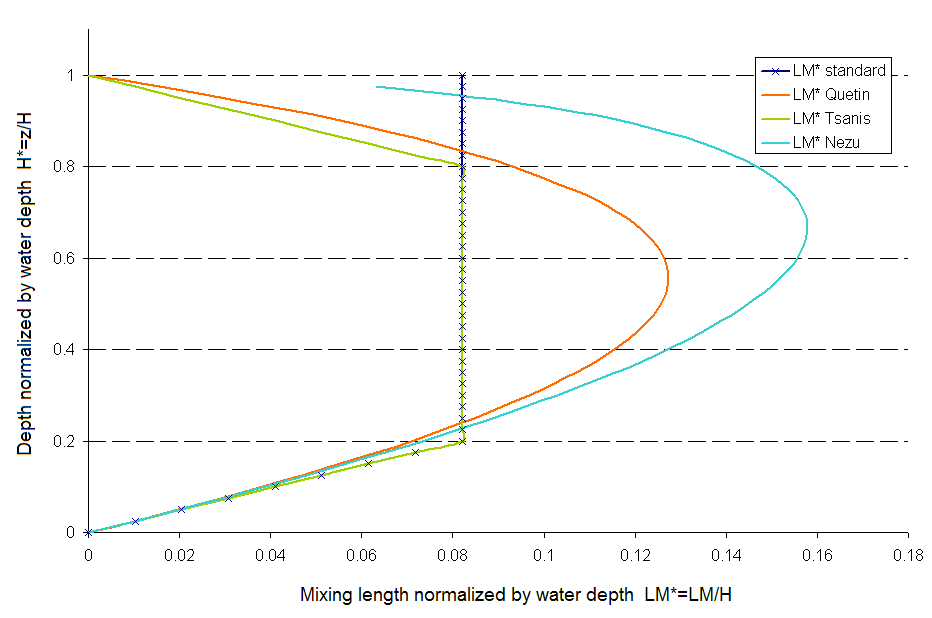
\includegraphics[width=\textwidth]{./graphics/mixing_lengths}
%
\end{center}
\caption
[Mixing lengths versus depth]
{Mixing lengths versus depth.}
\label{fig:mix_len}
\end{figure}

In the presence of a vertical density gradient, the environment stability
(respectively the instability) hinders (enhances) the vertical exchanges of
mass and momentum.

In order to quantify the effects of the gravity terms in the turbulent power
balance, the dimensionless Richardson number is commonly used. It is a local
number the value of which can obviously be different at each flow point.

In order to take the mixture reduction into a stable stratified flow into
account, a damping law is introduced into the turbulence model according to the
Richardson number. The user can set the damping function through the keyword
\telkey{DAMPING FUNCTION}. The available options are:

\begin{itemize}
\item  0: nothing (default value),

\item  1: user-performed; Law programming in the \telfile{DRIUTI} subroutine,

\item  2: Viollet,

\item  3: Munk and Anderson.
\end{itemize}

The graph below illustrates the variation of the Munk and Anderson damping
function according to the Richardson number for velocity and salinity. In the
case of a stable stratification, the pressure fluctuations more readily
transmit a momentum flux than a mass flux and the diffusion coefficient becomes
higher for the velocities than for the mass.

\begin{figure}[H]%
\begin{center}
%
  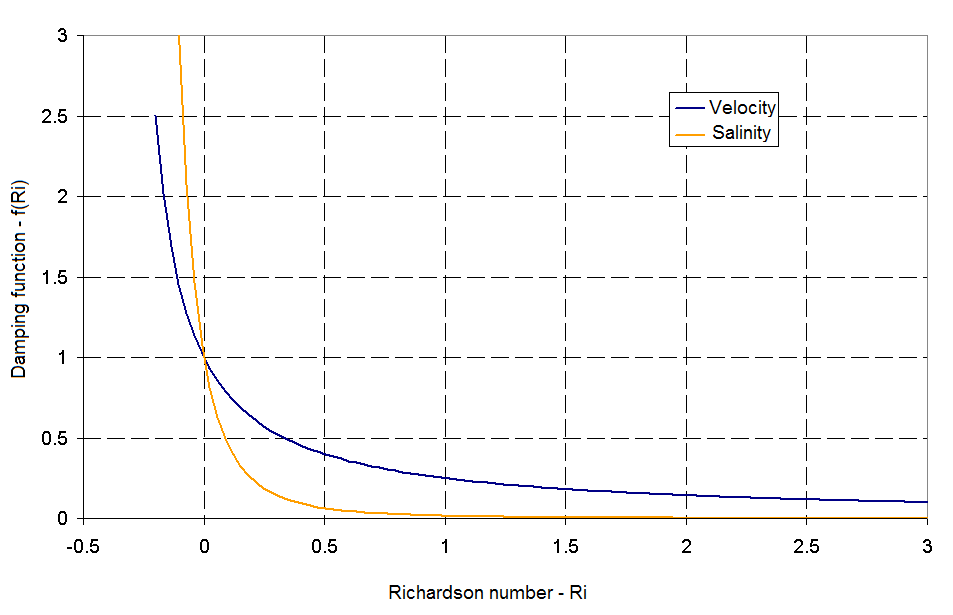
\includegraphics[width=\textwidth]{./graphics/munk_anderson}
%
\end{center}
\caption
[Munk and Anderson damping function]
{Munk and Anderson damping function.}
\label{fig:munk_anderson}
\end{figure}

When using the mixing length model, the user can also configure the calculation
of the vertical derivative of the velocities with the keyword \telkey{VERTICAL
VELOCITY DERIVATIVES}. Default value 1 corresponds
to a vertical derivative that is linear. Value 2 activates a logarithmic
computation between the bottom and 0.2 times the water depth. This allows
getting better results when modelling the velocity profile near the bottom.
This algorithm is implemented in the subroutine \telfile{VISCLM}.


\subsection{Smagorinsky}

That option is activated by setting the horizontal or vertical turbulence
model to 4 (Smagorinsky).

The Smagorinsky scheme is recommended, in particular, in the presence of a
highly non-linear flow \cite{Smagorinsky1963}.


\subsection{$k$-$\epsilon$}

\telemac{3D} gives an opportunity to use the so-called $k$-$\epsilon$
model as proposed by Rodi and Launder for solving the turbulence equations.
That model is activated by setting the keywords of turbulence models
(\telkey{HORIZONTAL TURBULENCE MODEL} and \telkey{VERTICAL TURBULENCE MODEL})
to the value 3.

The $k$-$\epsilon$ model is defined through a couple of equations
solving the balance equations for $k$ (turbulent energy) and $\epsilon$
(turbulent dissipation). Applying the $k$-$\epsilon$ model often
requires using a finer two-dimensional mesh than the constant viscosity model
and then increases the computation times.

For detailed information about the formulation of the mixing length and
$k$-$\epsilon$ models, the user can refer to the \telemac{3D} Theoretical
Note.

Strictly speaking, except for the constant viscosity model, the diffusion
coefficient should be equal to the molecular diffusion of water:

\begin{lstlisting}[language=TelemacCas]
COEFFICIENT FOR HORIZONTAL DIFFUSION OF VELOCITIES = 1.D-6
COEFFICIENT FOR VERTICAL DIFFUSION OF VELOCITIES = 1.D-6
\end{lstlisting}

The default value of that viscosity may have to be increased to ensure a minimum
diffusion, especially during the first time steps of the computation.

There are two options to compute the lateral boundary conditions of $k$ and
$\epsilon$ (in subroutine KEPCL3) with the keyword
\telkey{OPTION FOR THE BOUNDARY CONDITIONS OF K-EPSILON}:
\begin{itemize}
\item 1 = No turbulence ($k$ and $\epsilon$ takes the minimum values
\telfile{KMIN} and \telfile{EMIN} defined in subroutine \telfile{CSTKEP}),
which is the default value,
\item 2 = Hans and Burchard’s formula (introduced in version 7.0).
\end{itemize}

\section{Setting up the friction}

The bottom or sidewall friction reflects the continuity of the constraint at
the fluid-solid interface. Knowing the constraint involves knowing the flow in
the vicinity of the bottom. The turbulence models provide a modelling for that
flow.

The constraint can be written in several forms:
\begin{align}
\vec{\tau } & = \mu \frac{\partial \vec{U}}{\partial n}
            = -\frac{1}{2} \rho C_{f} \sqrt{U^{2} +V^{2} } \vec{U}\\
            & = -\rho U^{*2} 
\end{align}
where $U^{*}$ denotes the friction, $C_{f}$ - a dimensionless friction, $U$ -
the velocity of current recorded far enough from the wall.

The friction condition is then provided:

\begin{itemize}
\item  Either by a turbulence model which indicates the constraint through a
friction velocity formulation,

\item  Or by the knowledge of the friction coefficient $C_{f}$ and the related
velocity $U$ (here, the vertically-averaged velocity). That approach will then
use the Chézy, Strickler, Manning\dots  laws.
\end{itemize}

The same approach is adopted for both sidewalls and bottom.


\subsection{Bottom friction}

The friction law used for the bottom friction modelling is set by the keyword
\telkey{LAW OF BOTTOM FRICTION} which can assume the following values:

\begin{itemize}
\item  0: No friction,

\item  1: Haaland law,

\item  2: Chézy law (default value),

\item  3: Strickler law,

\item  4: Manning law,

\item  5: Nikuradse law.
\end{itemize}

As regards the 1-5 values, the value of the friction coefficient corresponds to
the selected law, and shall be given by means of the keyword \telkey{FRICTION
COEFFICIENT FOR THE BOTTOM}. Obviously, that only holds true if the friction is
constant in both space and time. The default value for that parameter is 60.

The computation of turbulent constraint at the bottom depends on the velocity
profile above the bottom (within the boundary layer). The profile depends on
the ratio of the wall asperity size to the viscous sub-layer thickness (for
further details, refer to the Theoretical Manual). When the asperities are
larger than the viscous sub-layer thickness, the latter cannot be established
and the friction regime is rough. On the other hand, when there is a viscous
sub-layer, the friction regime is smooth.

The computation of the turbulent constraint depends on the keyword
\telkey{TURBULENCE REGIME FOR THE BOTTOM}. The available options are:

\begin{itemize}
\item  1: smooth regime,

\item  2: rough (default value).
\end{itemize}

In smooth friction regime conditions,~the friction law is not used and the
constraint is computed from Reichard law of velocity profile (a law giving the
friction velocity value $U^{*}$.

In rough friction regime conditions and for the bottom friction laws 0, 2, 3
and 4, the constraint is computed from the friction velocity $U^{*}$ and its
relation to the $C_{f}$ coefficient. For law 5, the friction velocity is
computed from the velocity profile within the logarithmic layer and from the
asperity size $k_{s}$ (\telkey{FRICTION COEFFICIENT FOR THE BOTTOM}).


\subsection{Sidewall friction}

The friction law used to model the sidewall friction is set by the keyword
\telkey{LAW OF FRICTION ON LATERAL BOUNDARIES} which can take the following
values:

\begin{itemize}
\item  0: No friction (default value),

\item  5: Nikuradse law.
\end{itemize}

The size of asperities (which is used in the Nikuradse law) is given by the
\telkey{FRICTION COEFFICIENT FOR LATERAL SOLID BOUNDARIES} (default value 60!).

The friction is activated using the keyword \telkey{TURBULENCE REGIME FOR
LATERAL SOLID BOUNDARIES}. The available options are:

\begin{itemize}
\item  1: smooth regime,

\item  2: rough (default value).
\end{itemize}

That option changes the formulation of the velocity profile and consequently,
the friction velocity. See previous section for more information.

\section{Punctual source terms}
\label{sec:srcfile}
\telemac{3D} offers an opportunity to place momentum sources or sinks in any
point of the domain.

The user places horizontally the various sources using the keywords
\telkey{ABSCISSAE OF SOURCES} and \telkey{ORDINATES OF SOURCES}. They are
arrays of reals giving the co-ordinates of sources, in meters. Actually,
\telemac{3D} will position a source at the closest mesh point to the point as
specified by these keywords. The software will determine itself the number of
source according to the number of values given to each keyword.

The vertical positioning of the sources is done using the keyword
\telkey{ELEVATIONS OF SOURCES}. \telemac{3D} places the sources on the nearest
mesh level. In this case, it is recommended to use fixed levels at sources
elevations in order to avoid unwanted vertical movement of the sources during
the simulation. Also note that the sources cannot be placed on the bottom level
(level number 1). This is to ensure an impermeable bottom boundary.

At each source, the user should specify the liquid flow rate. That liquid flow
rate is given (in m${}^{3}$/s) using the keyword \telkey{WATER DISCHARGE OF
SOURCES}.

In case of sources with variable characteristics, the user can then either use
specific programming in the \telfile{T3D\_DEBSCE} subroutine (and
\telfile{T3D\_TRSCE} in the presence of tracer), or use the source file whose
name is given by the keyword \telkey{SOURCES FILE}.
This file has exactly the same structure as the liquid
boundary file. An example is shown below with two sources and two tracers.
Between two specified times, the information used by \telemac{3D} at sources is
obtained by linear interpolation.

\begin{lstlisting}[language=TelemacCas]
#
#  FLOW RATES ANS TRACERS CONCENTRATIONS AT SOURCES 1 ET 2
#
#  T IS THE TIME
#
#  Q(1) IS FLOW RATE AT SOURCE 1
#  Q(2) IS FLOW RATE AT SOURCE 2
#
#  TR(1,1) IS TRACER 1 CONCENTRATIONS AT SOURCE 1
#  TR(1,2) IS TRACER 2 CONCENTRATIONS AT SOURCE 1
#  TR(2,1) IS TRACER 1 CONCENTRATIONS AT SOURCE 2
#  TR(2,2) IS TRACER 2 CONCENTRATIONS AT SOURCE 2
#
#
T     Q(1)     TR(1,1)    TR(1,2)    Q(2)      TR(2,1)   TR(2,2)
s     m3/s        C          C        m3/s        C         C
0.     0.        99.        20.       0.         30.       40.
2.     1.        50.        20.       2.         30.       20.
4.     2.        25.        80.       4.         30.       20.
\end{lstlisting}

Besides, \telemac{3D} is capable of taking into account an injection velocity (in
m/s) at the sources in the dynamic equations. By default, the injection takes
places without any momentum input. The user may prescribe a particular
velocity. If the latter is constant throughout the simulation, then its value
can be given using the keywords \telkey{VELOCITIES OF THE SOURCES ALONG X},
\telkey{VELOCITIES OF THE SOURCES ALONG Y} and
\telkey{VELOCITIES OF THE SOURCES ALONG Z}. Otherwise, the user
should program the SOURCE subroutine in order to amend \telfile{USCE} (for the
velocity at sources along $X$) and \telfile{VSCE} (for the velocity at sources
along $Y$). The user can use the time and all the parameters of the sources
within that subroutine.

From a theoretical point of view, complete mass conservation can only be ensured
if the source is treated as a Dirac function and not as a linear function.
The type of treatment is indicated by the user with the keyword
\telkey{TYPE OF SOURCES}, which can have a value of 1 (linear function,
default value) or 2 (Dirac function).
It should be noted that in the second case, the solutions are of course
less smoothed.
It is the same implementation as in \telemac{2D} and the Dirac option is
recommended with a big number of sources.
The maximum number of sources is set to 20 by default but it can be changed
by the user with the keyword \telkey{MAXIMUM NUMBER OF SOURCES}.
This avoids changing the previously hardcoded values (until version 7.0),
which required recompiling the whole package.

\section{Setting up the water-atmosphere exchanges}

\subsection{The wind}

\telemac{3D} can be used to simulate flow while taking into account the influence
of a wind blowing on the water surface. The logical keyword \telkey{WIND} is
used first of all for determining whether this influence is taken into account
and if so, the coefficient is then provided with the keyword
\telkey{COEFFICIENT OF WIND INFLUENCE}(see next subsection). Lastly, if the
wind is constant in time and space, wind speed in directions X and Y is
supplied with the keywords \telkey{WIND VELOCITY ALONG X} and \telkey{WIND
VELOCITY ALONG Y}. Default values for these three coefficients are 0.

The coefficient of wind influence hides complex phenomena. In fact, the
influence of the wind depends on the smoothness (or, lack of it) of the free
surface and the distance over which it acts (called the ``fetch''). The
coefficient value can be obtained from many different formulas.

This is the formula used by the Institute of Oceanographic Sciences (United
Kingdom):

\begin{tabular}{ll}
if $\overrightarrow{U}_{vent} < 5$ m/s & $a_{vent}  = 0.565 \times 10^{-3}$ \\
if $5 < \overrightarrow{U}_{vent}  < 19.22$ m/s & $a_{vent} = (- 0.12 + 0.137\overrightarrow{U}_{vent} ) 10^{-3}$ \\
if $\overrightarrow{U}_{vent} > 19.22$ m/s & $a_{vent} = 2.513 \times 10^{-3}$ \\
\end{tabular}

The parameter \telkey{COEFFICIENT OF WIND INFLUENCE} asked for by \telemac{3D}
is: $a_{vent} (\rho_{air} / \rho)$ and not only $a_{vent}$.
$\rho_{air}$ is approximately 1.2 kg/m$^3$ and $\rho$
is approximately 1,000 kg/m$^3$. Thus it is necessary to divide the value of
$a_{vent}$ by 1,000 to obtain the value of the \telemac{3D} keyword.

The whole formulation used to consider the wind effects, through the keyword
\telkey{COEFFICIENT OF WIND INFLUENCE} (refer to the Theoretical Note for the
definition of that coefficient), on the surface flows is fully stated in the
\telfile{BORD3D} subroutine.

If the wind velocity is space- or time-variable, the user should modify the
\telfile{METEO} subroutine.

\begin{WarningBlock}{Warning:}
The \telfile{METEO} subroutine is provided to define the wind velocity and
direction even though they are space- or time-variable.
The \telfile{BORD3D} subroutine describes the law of wind-induced drift
of water bodies.
\end{WarningBlock}

If there are tidal flats or dry zones in the domain, the wind may trigger
unphysical velocities as it becomes the only driving term in the equations. To
avoid this, the influence of the wind is cancelled below a threshold value of
depth, with the key-word \telkey{THRESHOLD DEPTH FOR WIND} (default value at
1~m).


\subsection{The temperature}

Air temperature may be specified using the keyword \telkey{AIR TEMPERATURE} if
it is constant in time and space.


\subsection{The pressure}

The influence of air pressure is taken into account from the moment when the
keyword \telkey{AIR PRESSURE} is set to YES (the default value is
NO). The value of that pressure is directly set in the \telfile{METEO} subroutine.
By default, the latter initializes a pressure of $10^5$ Pa ($\approx$ 1 atm) over
the whole domain.


\subsection{Rain or evaporation}

The modelling of the influence of precipitation or evaporation is activated
with the logical keyword \telkey{RAIN OR EVAPORATION}. The value of the
contribution or the loss of water at the surface is specified using the keyword
\telkey{RAIN OR EVAPORATION IN MM PER DAY} which default value is 0. (a
negative value reflects an evaporation).

In case of calculation with consideration of tracers, it is possible to specify
the contribution related to the rain with the keyword \telkey{VALUES OF TRACERS
IN THE RAIN} (default value is 0.). It is important to note that, in the case
of evaporation, no tracer is taken into account in the water loss, which is
incorrect if the tracer is the temperature.

\subsection{Atmosphere-water exchange models}

Before version 7.0, heat exchange between water and atmosphere could have been
done with a linearised formula of the balance of heat exchange fluxes at the
free surface. An example of an exchange with a constant atmosphere temperature
and a constant sea salinity was given as standard (as comments) through a
direct programming in the \telfile{BORD3D} subroutine.

A much more elaborated model has been introduced in \telemac{3D}. This module
calculates the complete balance of exchanged fluxes involved:

\begin{itemize}
\item  The solar radiation,

\item  The atmospheric radiation,

\item  The water radiation,

\item  The latent heat due to evaporation,

\item  The sensitive heat of conductive origin.
\end{itemize}

It takes into account the solar radiation penetration in the water column.

The choice of the heat exchange model can be done with the keyword
\telkey{ATMOSPHERE-WATER EXCHANGE MODEL} (default value = 0: no exchange
model). Value 1 will use with the linearised formula at the free surface,
whereas value 2 will use with the model with complete balance.

These calculations require additional data (wind magnitude and direction, air
temperature, atmospheric pressure, relative humidity, nebulosity and rainfall,
all these variables may vary in time) in a standard format, see the example
"heat\_exchange". The format may be changed but the user has to change the
implementation of the reading and the interpolation of the meteorological data.
When using the complete module, evaporation is calculated by \telemac{3D}, but
the user has to provide rainfall data with units homogeneous with length over
time.

The main developments of this module are implemented in the module
\telfile{EXCHANGE\_WITH\_ATMOSPHERE}.

Some physical parameters have been hard-coded in the module, often imposed as
the mean value: the type of sky related to the luminosity of the site (very
pure sky, mean pure sky or industrial zone sky), the type of cloud (cirrus,
cirro stratus, alto cumulus, alto stratus, stratus), but these values can be
changed in the module \telfile{EXCHANGE\_WITH\_ATMOSPHERE}).

Because the site of a study may not be equipped with local wind measurements
and these kinds of data are available at a different location, possibly far
from the studied site, a wind function is used. This is a linear function with
a single coefficient of calibration $b:f(U_{2}) = b(1+U_{2}$) where $U_{2}$ is
the wind velocity at 2~m high.

To get the wind velocity at 2~m high from classical wind data at 10~m high, a
roughness length of ${z}_{0}~=~0.0002$~m has been chosen in the code,
that leads to $U_{2} \approx 0.85 U_{10}$. This value
of 0.85 (or the roughness length) may be changed by the user if needed.

Examples of solar radiation penetration are given in comments in the
\telfile{SOURCE\_TRAC} subroutines. Two laws are suggested: the first one
uses the \emph{in situ} measurements of Secchi length and is
recommended if available; the second one uses two exponential laws that may be
difficult to calibrate and require an estimation of the type of water from
turbidity.

Except for the coefficient to model the penetration of solar radiation in the
water column, the parameter $b$ that appears in the wind function is the
single calibration parameter of this module. Its value is given by the keyword
\telkey{COEFFICIENT TO CALIBRATE THE ATMOSPHERE-WATER EXCHANGE MODEL}. (default
value = 0.0025 but recommended values are between 0.0017 and 0.0035). This
keyword is both used for the linearised formula at the free surface and the
model with complete balance (values 1 and 2 for the keyword
\telkey{ATMOSPHERE-WATER EXCHANGE MODEL}).


\section{Astral potential}

When modelling large maritime areas, it is sometimes necessary to take into
account the effect of astral forces generating tide inside the area. For this,
the user has several keywords at his disposal.

First of all, the logical keyword \telkey{TIDE GENERATING FORCE} (default value
NO) allows these phenomena to be taken into account.

The keyword \telkey{LONGITUDE OF ORIGIN POINT} must be positioned at the right
value.

Lastly, the two keywords \telkey{ORIGINAL DATE OF TIME} (format YYYY;MM;DD) and
\telkey{ORIGINAL HOUR OF TIME} (format HH;MM;SS) must be used to give the
beginning time of the simulation.  This information is necessary for \telemac{3D}
to compute the respective position of the moon and the sun.

\section{Consideration of wave driven currents}

It is possible to take into account the wave driven currents by retrieving
information calculated by a wave propagation module of the TELEMAC modelling
system (mainly \tomawac but also \artemis). In the current version,
only taking into account a steady state is possible. The procedure is as
follows:

\begin{itemize}
\item  Perform a calculation of wave propagation on the same mesh as the
\telemac{3D} calculation requesting the storage of the driving forces. In the
case of \tomawac, the variables \telfile{FX} and \telfile{FY},

\item  Get the wave results file and provide its name through the keyword
\telkey{BINARY DATA FILE 1},

\item  Activate the keyword \telkey{WAVE DRIVEN CURRENTS},

\item  Fill the keyword \telkey{RECORD NUMBER IN WAVE FILE}. This value
corresponds to the iteration number stored in the wave file which must be taken
into account by \telemac{3D}. Usually, this is the last iteration stored, by
default this number is set to 1. The name of the variables to read is "FORCE
FX" and "FORCE FY", but this can be changed within the TRISOU subroutine.
\end{itemize}

In the current version of \telemac{3D}, this driving force is considered as being
constant over the vertical.

If the user wishes to take into account several results of the wave propagation
module (e.g. to take into account changes in the level of the sea), FORTRAN
programming is required.

\section{Other physical parameters}

When modelling large domains, the influence of the Coriolis force of inertia
has to be taken into account. This is done by activating the logical keyword
\telkey{CORIOLIS} (which is set to NO by default). In such a case, the value of
the Coriolis coefficient (refer to the Theoretical Note) is defined by the
keyword \telkey{CORIOLIS COEFFICENT} (default value is 0.). The latter should
be computed according to latitude l through the formula:

\begin{itemize}
\item  $2\, \omega \, \sin \, \left(\lambda \right)$ where $\omega$ is the
Earth's rotational velocity of $7.27 \times {10}^{-5}$ rad/s and $\lambda$ is the
average latitude of the model.
\end{itemize}

In the case of very large domains such as portions of oceans, it is necessary
to carry out a simulation with spherical coordinates, in which case the
Coriolis coefficient is adjusted automatically at each point of the domain (see
10.3), by activating the keyword \telkey{SPHERICAL COORDINATES}.

\telemac{3D} additionally offers the opportunity to set the acceleration due to
gravity (keyword \telkey{GRAVITY ACCELERATION} which, by
default, is set to 9.81~m/s${}^{2}$).
